%%%%%%%%%%%%%%%%%%%%%%%%%%%%%%%%%%%%%%%%%%%%%%%%%%%%%%%%%%%%%%%%%%%%%%%%
%                                                                      %
%     File: Thesis_Implementation.tex                                  %
%     Tex Master: Thesis.tex                                           %
%                                                                      %
%     Author: João D. Lopes                                            %
%     Last modified :  7 July 2017                                     %
%                                                                      %
%%%%%%%%%%%%%%%%%%%%%%%%%%%%%%%%%%%%%%%%%%%%%%%%%%%%%%%%%%%%%%%%%%%%%%%%

\chapter{Architecture}
\label{chapter:architecture}

Versat is designed for fixed-point signal processing and its
architecture is shown in figure~\ref{fig_top}. It can be used by host
processors in the same chip, as some procedures can run faster and at
lower energy on Versat.

In order to reduce the dependency on the host CPU, Versat features a
simple Controller used for algorithmic control, self-reconfiguration
and data movement. This frees the host for more useful tasks. The
controller is programmable and has an instruction memory where Versat
programs (aka kernels) are stored. Control over the different modules
is exerted using a Control Bus. Though not shown, there is also a
serial divider accessible from the Control Bus.

Versat has a special unit that performs data computation, the Data
Engine (DE). This unit is composed of Functional Units (FUs)
interconnected by a full mesh. Hence, there is more than one way to
make a given datapath, which is useful for simplifying the compiler.

The Configuration Module (CM) holds the configuration of the DE, i.e.,
it specifies the current datapath, and has another register where the
next configuration of the DE can be prepared; it can also temporarily
store tens of other complete configurations, which can be switched at
runtime. The Controller can write partial configurations to the CM,
and can also save and restore entire configurations from the
configuration memory.

\begin{figure}[!htb]
\centering 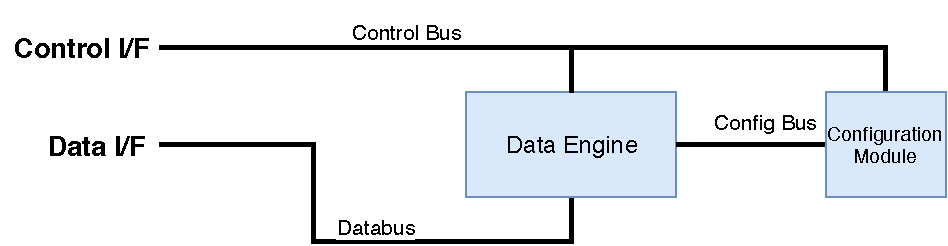
\includegraphics[width=0.70\textwidth]{drawings/top.pdf}
\caption{Versat top-level entity.}
\label{fig_top}
\end{figure}

Versat has a DMA module so it can independently and efficiently
transfer data, programs and configurations in and out of the
device. The DMA drives a master Advanced Extensible Interface --
AXI4. It is an interface designed by ARM, which derives from the
Advanced Microcontroller Bus Architecture (AMBA).

To communicate with the host processor, Versat has a shared Control
Register File (CRF). The CRF has two host interfaces that can be
selected at compile time: a Serial Peripheral Interface (SPI) and a
parallel bus interface. The SPI slave interface is used when the host
system is an off-chip master device. The SPI interface is mainly used
for debug and testing purposes. The parallel bus interface is used
when the host is some embedded processor and may be supplied in the
AXI4 Lite format.


%%%%%%%%%%%%%%%%%%%%%%%%%%%%%%%%%%%%%%%%%%%%%%%%%%%%%%%%%%%%%%%%%%%%%%%%
\section{Data Engine}
\label{section:dataEngine}

The Data Engine (DE) has a fixed topology comprising 15 Functional
Units (FUs) as shown in figure~\ref{fig_de}. The DE is a 32-bit
architecture and contains the following configurable FUs: 4 dual-port
embedded memories ($8kB$ each), 6 Arithmetic and Logic Units (ALUs), 4
multipliers and 1 barrel shifter. The output register of the FUs and
the embedded memories are accessible by the Controller for reading and
writing. (The embedded memory blocks are treated like any other FU by
the Versat tools.)

\begin{figure}[!htb]
\centering
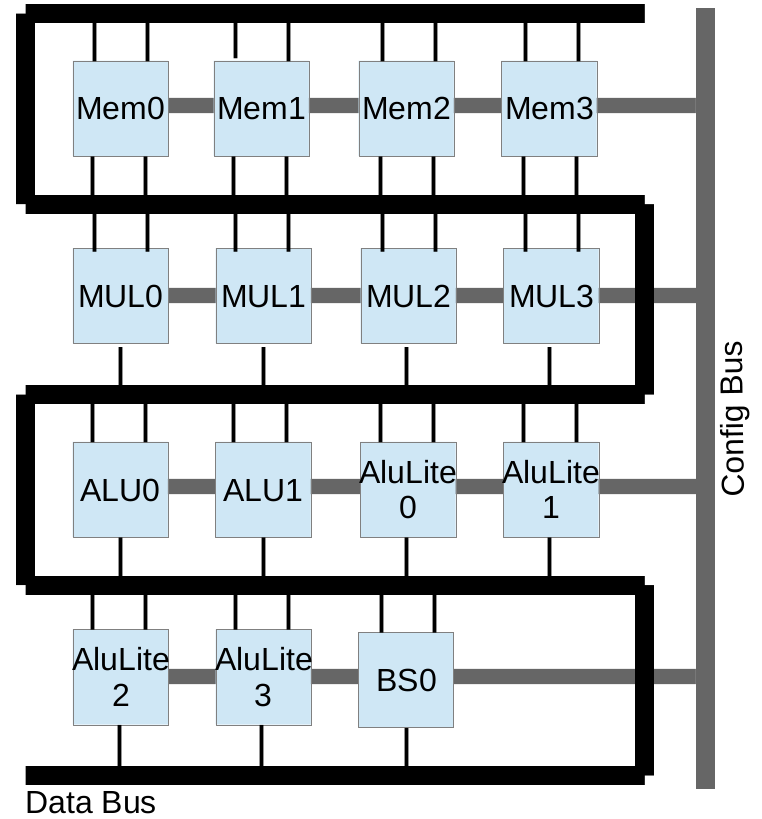
\includegraphics[width=0.75\textwidth]{drawings/de.pdf}
\caption{Data engine.}
\label{fig_de}
\end{figure}

\subsection{DE Structure}
\label{subsection:DEStructure}

In the DE, the FUs are interconnected by a wide bus called the Data
Bus. The Data Bus is simply the concatenation of all FU outputs. Each
FU output contributes a 32-bit section to the Data Bus, except the
embedded memories that contribute 2 sections with their 2
ports. According to the number of FUs of each type given before, the
Data Bus has $2\times4+6+4+1=19$ sections of 32 bits. In addition to
FU outputs, the Data Bus has 2 fixed sections containing the constants
0 and 1, which have been added because they are commonly used in
datapaths. Each FU input can select any of these sections and there is
also a selection that ignores the input value so that FU can be used
as a Controller shared register. The FUs take their configurations
from the respective configuration registers in the CM, whose outputs
are concatenated in another wide bus denoted the Config Bus. There is
a fixed set of high-level operations available in each FU. For
example, an ALU can be configured to perform addition, subtraction,
several logical functions, maximum, minimum, among others.

In figure~\ref{fig_fu}, it is shown in detail how a particular FU is
connected to the control, data and configuration buses. The FU, of
type ALU, is labeled FU5 and has 2 pipeline stages. The last pipeline
stage, denoted {\tt pipeline register 1}, stores the output of the
ALU, drives one section of the Data Bus and can be read or written by
the Controller using the Control Bus (as shown in the figure). This
feature enables the FUs to be used as Controller/DE shared
registers. Each FU5 input has a programmable multiplexer to select one
of the 19 sections of the Data Bus. Although the Config Bus is shown
going to all FUs, in fact only the configuration bits of each FU are
routed to it. These bits are called the {\em configuration space} of
the FU. The configuration space is further divided in several {\em
  configuration fields}, which are 3 in this example: the selection of
input A (5 bits), the selection of input B (5 bits) and the selection
of the function (4 bits). The partial reconfiguration scheme works at
the field level, so it is only possible to reconfigure these fields
individually.

\begin{figure}[!htb]
\centering
\includegraphics[width=0.85\textwidth]{drawings/FU.pdf}
\caption{Functional unit detail.}
\label{fig_fu}
\end{figure}

Since any FU can select any FU output as one of its inputs, then the
DE has a {\em full mesh topology}. This may seem exaggerated and
unnecessary but this topology accomplishes 2 major goals: (1) {\em an
  intuitive assembly programmer's model is achieved}; (2) {\em the
  compiler design is greatly simplified}. In fact, assembly
programmers need not remember or check what is connected to what since
everything is connected to everything. Hardware datapaths can be
manually built using store instructions that write to the
configuration fields of the used FUs. A compiler can be developed with
less effort as complex place and route algorithms, commonly used in
CGRAs, become unnecessary with a fully connected topology.

Assembly programmability is a powerful feature. It may be used to
optimize critical program sections or to work around bugs. In fact,
hardware bugs, defects or failures may eventually be circumvented at
post-silicon time using assembly code to avoid using the troubled
parts of the architecture. Compiler problems can also be fixed by
replacing the failing high-level code with assembly code.

In other approaches, such as in~\cite{Mei05}, a full mesh topology
would be problematic because of the cycle by cycle reconfiguration. It
causes frequent switching of the interconnect network and consequent
power dissipation. However, in Versat, reconfiguration does not happen
every clock cycle. The interconnect consumes very little power since
Versat is reconfigured only after a complete program loop or two
levels of nested loops are executed in the DE. It may also be argued
that a full mesh topology is large and limits the frequency of
operation. However, our IC implementation results indicate that only
$4.04\%$ of the core area is occupied by the full mesh interconnect,
while the core can work at a maximum frequency of $170MHz$ in a
$130nm$ process. This is sufficient for many target applications. For
example, in the multimedia space, some applications are required to
work at an even lower frequency because of power and energy
constraints.

Each configuration of the DE can implement one or more hardware
datapaths. Multiple datapaths operating in parallel realize
Thread-Level Parallelism (TLP). Datapaths having identical parallel
paths implement Data-Level Parallelism (DLP). Finally, datapaths
having long FU pipelines exploit Instruction-Level Parallelism (ILP).

In figure~\ref{fig_de_dp}, three example hardware datapaths are
illustrated. Datapath (a) implements a pipelined vector
addition. Despite the fact that a single ALU is used, ILP is being
exploited as the memory reads, addition operation and memory write are
being executed in parallel for consecutive elements of the
vector. Datapath (b) implements a vectorized version of datapath (a)
to illustrate DLP combined with the ILP. The vectors to be added
spread over memories M0 and M2, so that 2 additions can be performed
in parallel. ILP and DLP can be further exploited as in datapath (c),
whose function is to compute the inner product of two vectors: four
elements are multiplied in parallel and the results enter an adder
tree with an accumulator at the root. When an ALU is used as an
accumulator the unused data input is used as a control input. As seen
in the figure, this input is kept with the value 0, which specifies
the accumulator function. Any positive value specifies this function
while a negative value specifies that the ALU simply registers the
data input.

\begin{figure}[!htb]
\centering
\includegraphics[width=0.85\textwidth]{drawings/datapaths.pdf}
\caption{Data engine datapaths.}
\label{fig_de_dp}
\end{figure}


%%%%%%%%%%%%%%%%%%%%%%%%%%%%%%%%%%%%%%%%%%%%%%%%%%%%%%%%%%%%%%%%%%%%%%%%
\subsection{Address Generation Unit}
\label{subsection:addressGenerationUnit}

Versat has 4 dual-port Random Access Memories (RAMs) of size 2048
words by 32 bits, which work normally as vector registers. Each port
has an input, an output and an address input equipped with an Address
Generation Unit (AGU), as shown in figure~\ref{fig_dpram}. The AGUs
can be programmed to generate an address sequence for accessing data
from the memory port during the execution of a program loop. Our AGU
scheme is similar to the one described in~\cite{Farahini14}, in the
sense that both schemes use parallel and distributed AGUs. The AGUs
support two levels of nested loops, with the restriction that the
inner loop has a maximum of 32 iterations and the outer loop has a
maximum of 2048 iterations. To compute longer loops reconfiguration is
needed. AGUs can start execution with a programmable delay, so that
circuit paths with different accumulated latencies can be
synchronized. Each AGU can be operated independently from the other
AGUs, which allows TLP in the DE.

\begin{figure}[!htb]
\centering
\includegraphics[width=0.45\textwidth]{drawings/dpram.pdf}
\caption{Dual-port embedded memory with AGUs.}
\label{fig_dpram}
\end{figure}

Datapath (b) in figure~\ref{fig_de_dp}, previously used to explain
DLP, can also be used to explain TLP as follows. Suppose one block of
vector elements to be added is placed in memory M0, and that its
address generators M0-A, M0-B and M1-A are started (Thread 1). In
parallel, one can move the next block to memory M2 and start AGUs
M2-A, M2-B and M1-B (Thread 2). The user program can monitor the
completion of these threads and restart them with new vector
blocks. In this way, vectors that largely exceed the capacity of the
DE memories can be processed in a continuous fashion.

\begin{table}[!htb]
  \renewcommand{\arraystretch}{1.2} % more space between rows
  \caption{Address generation unit parameters.}
  \label{tab:MemParameter}
  \centering
  \begin{tabular}{lcp{10cm}}
    \toprule
    Parameter & Size (bits) & Description\\
    \midrule
    Start     &          11 & Memory start address. Default value is 0. \\
    Per       &           5 & Number of iterations of the inner loop, aka Period. Default is 1 (no inner loop). \\
    Duty      &           5 & Number of cycles in a period (Per) that the memory is enabled. Default is 1.\\
    Incr      &          11 & Increment for the inner loop. Default is 0.\\
    Iter      &          11 & Number of iterations of the outer loop. Default is 1.\\
    Shift     &          11 & Additional increment in the end of each period. Note that Per+Shift is the increment of the outer loop. Default is 0.\\
    Delay     &           5 & Number of clock cycles that the AGU must wait before starting to work. Used to compensate different latencies in the converging branches of the configured hardware datapaths. Default is 0.\\
    Reverse   &           1 & Bit-wise reversion of the generated address. Certain applications like the FFT work with mirrored addresses. Default is 0.\\
    \bottomrule
  \end{tabular}
\end{table}

The AGU parameters control the generation of address sequences and are
described in~Table~\ref{tab:MemParameter}. With these parameters the
AGU can generate an address sequence for an embedded memory port. An
example address sequence is shown in figure~\ref{fig_addrgen}. Note
that the AGU is enabled with a Delay of 2 clock cycles. It is enabled
periodically for $Duty=3$ cycles after every $Per=5$ cycles. The
initial value of the sequence is given by $Start=10$ (in decimal
notation). Every enabled cycle it is incremented by $Incr=2$; in the
last cycle of a period it is incremented by $Incr+Shift=-3$. This
pattern repeats for $Iter$ iterations, though this parameter is not
illustrated in the figure.

\begin{figure}[!htb]
\centering
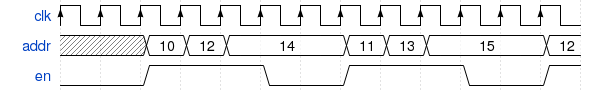
\includegraphics[width=0.75\textwidth]{drawings/addrgen.png}
\caption{AGU output for $Delay=2$, $Per=5$, $Duty=3$, $Start=10$, $Incr=2$, and $Shift=-5$.}
\label{fig_addrgen}
\end{figure}

The embedded memory ports have their own configuration fields: one for
selecting/disabling the input or outputting the generated sequence
(sel) and another for bypassing the AGU (Ext). If the input is
disabled then the port is enabled for reading. If it is selecting a
data source, then it is enabled for writing but also reads the word
previously stored at that address. Normally an AGU is used for
generating an address sequence for the memory port. However, the port
can also be configured to output the generated sequence to the DE,
where it can be used for general purposes. With this feature, data
patterns, synchronization and control signals can be generated for the
FUs. The configuration for bypassing the AGU ($Ext=1$) enables the
port to use as address values computed by datapath. In this case the
port address is input by the other port of the same memory. This
feature provides Versat with the capability of working with pointers.

In summary, the two memory ports can be independently configured to
read and/or write the memory, each memory port can be read/written with
an address sequence computed by the AGU or by some datapath in the
DE, and a memory configured for writing also reads the previously
stored word from the same address with one clock cycle of latency.

%%%%%%%%%%%%%%%%%%%%%%%%%%%%%%%%%%%%%%%%%%%%%%%%%%%%%%%%%%%%%%%%%%%%%%%%
\subsection{Arithmetic and Logic Unit}
\label{subsection:arithmeticLogicUnit}

There are two types of Arithmetic and Logic Units (ALUs), denoted Type
I and Type II: 2 Type I and 4 Type II. Both types have two inputs, A
and B, and an output Y.  A summary of the ALU operations is given in
Table~\ref{tab:AluOpers}. The ALUs have 4 configuration bits for the
operation field and thus can support 16 different operations.

\begin{table}[!htb]
  \renewcommand{\arraystretch}{1.2} % more space between rows
  \caption{ALU functions.}
  \label{tab:AluOpers}
  \centering
  \begin{tabular}{lll}
    \toprule
    Operation              &                Type I & Type II (w/ feedback)\\
    \midrule
    Logic OR               &           Y = A $|$ B & Y = Y $|$ B\\
    Logic AND              &            Y = A \& B & Y = Y \& B\\
    Logic XOR              &      Y = A $\oplus$ B & NA\\
    Addition               &             Y = A + B & Y = (A$<$0)? B: Y+B\\
    Subtraction            &             Y = B - A & Y = (A$<$0)? B: Y-B\\
    Multiplexer            &     Y = (A$<$0)? B: 0 & Y = (A$<$0)? B: Y\\
    Sign extend 8          &    Y = A[7]...A[7..0] & NA\\
    Sign extend 16         &  Y = A[15]...A[15..0] & NA\\
    Shift right arithmetic & Y = {A[31], A[31..1]} & NA\\
    Shift right logical    &   Y = {'0', A[31..1]} & NA\\
    Signed compare         &       Y[31] = (A$>$B) & Y[31] = (Y$>$B)\\
    Unsigned compare       &       Y[31] = (A$>$B) & NA\\
    Count lead zeros       &            Y = CLZ(A) & NA\\
    Signed maximum         &            Y=max(A,B) & Y = (A$<$0)? Y: max(Y,B)\\
    Signed minimum         &            Y=min(A,B) & Y = (A$<$0)? Y: min(Y,B)\\
    Absolute value         &             Y=$|$A$|$ & NA\\
    \bottomrule
  \end{tabular}
\end{table}

Type II ALUs use one of the configuration bits to create an internal
feedback loop from the output to input A. With the other 3 bits, Type
II ALUs can support 8 operations. If the feedback bit is set to '0',
these operations are the same as for Type I ALUs. If the feedback bit
is set to '1', the operation has input B and the current output as
operands. In this case, input A becomes available for runtime control
of the ALU, which is used for implementing conditional statements in
operations ADD, SUB, MUX, MIN and MAX. For instance, the addition
operation (ADD) can be turned into a conditional accumulate operation:
the ALU accumulates the values coming to input B, if input A is not
negative or simply registers input B otherwise. In another example,
the signed minimum operation can be used to detect and register the
minimum value among only certain elements of a sequence coming to
input B, by using input A as a data qualifier. Often, an AGU is used
to generate control sequences for the control input A of an ALU. The
type II ALU is an original way to enable conditional execution in the
DE.

%%%%%%%%%%%%%%%%%%%%%%%%%%%%%%%%%%%%%%%%%%%%%%%%%%%%%%%%%%%%%%%%%%%%%%%%
\subsection{Multiplier and Barrel Shifter}
\label{subsection:multiplierBarrelShifter}

The multiplier produces a 64-bit result from two 32-bit operands and
has two configuration parameters. One parameter allows selecting the
lower or higher 32 bits of the result. The other parameter forces the
multiply result to be left shifted by 1 bit. This configuration is
useful when operands are in the Q1.31 fixed-point format, which is
used in many DSP algorithms. By setting the first parameter to select
the high part of the result and the second parameter to left shift it
by 1, the multiplication of two Q1.31 operands also yields a Q1.31
result.

The barrel shifter can perform left and right shifts. Right shifts can
be configured as logical (no sign extension, feed '0' to the left) or
arithmetic (with sign extension). One configuration parameter
determines the shift direction (left or right) and another parameter
sets the right shift type (arithmetic or logic). In one input of the
barrel shifter is the value to be shifted and in the other input is
the shift size (0 to 31).

%%%%%%%%%%%%%%%%%%%%%%%%%%%%%%%%%%%%%%%%%%%%%%%%%%%%%%%%%%%%%%%%%%%%%%%%
\subsection{Functional Unit Latencies}
\label{subsection:functionalUnitLatencies}

Each FU has a latency due to pipelining: 2 clock cycles for the ALUs,
3 for the multipliers and 1 for the barrel shifter and embedded
memories. When configuring a datapath in the DE, it is necessary to
take into account the latency of each branch, and compensate for any
mismatches when branches with different latencies converge. To do
this, the AGUs have the {\em Delay} parameter explained in
Table~\ref{tab:MemParameter}. The branch latency is the sum of its FU
latencies.

%%%%%%%%%%%%%%%%%%%%%%%%%%%%%%%%%%%%%%%%%%%%%%%%%%%%%%%%%%%%%%%%%%%%%%%%
\subsection{Data Engine Control}
\label{subsection:dataEngineControl}

The DE is controlled using its Control and Status registers. The
Control register structure is the following: bit 0 (init) resets the
selected memory ports and bit 1 (run) enables the selected ports,
resets the selected FUs and starts the DE; bits~2~-~20 select the
memory ports and FUs to reset or enable. Recall there are 8 memory
ports and 11 other FUs in a total of 19 FUs to control. The Status
register structure is the following: bits~0~-~7 indicate which AGUs
are running (logic '0') or idle (logic '1').

%%%%%%%%%%%%%%%%%%%%%%%%%%%%%%%%%%%%%%%%%%%%%%%%%%%%%%%%%%%%%%%%%%%%%%%%
\section{Configuration Module}
\label{section:configuration}

The Configuration Module (CM) is composed of a Configuration Register
File used to prepare the next configuration, the Configuration Shadow
Register which holds the configuration being executed by the DE, and
the Configuration Memory where frequently used configurations are
stored (figure~\ref{fig_conf}). Configurations stored in the
configuration memory can later be used without modifications or they
can be partially reconfigured before used.

The configuration register file is divided in configuration spaces
which in turn are divided in configuration fields. Different
configuration spaces differ on the number of fields and configuration
fields differ on the number of bits. A full DE configuration is 672
bits. The configuration register file is addressable at the
configuration field level and there are 118 configuration fields. This
feature takes advantage of the fact that in most applications there is
a high likelihood that a certain configuration or a similar one will
be reused (time locality) to make partial reconfiguration effective.

The configuration shadow register holds an active configuration word
for the DE, which is copied from the configuration register file
whenever the Update signal is asserted by the Controller. Thus, the
contents of the configuration register file can be changed while the
configuration shadow register keeps the DE configured and running.

\begin{figure}[!htb]
\centering 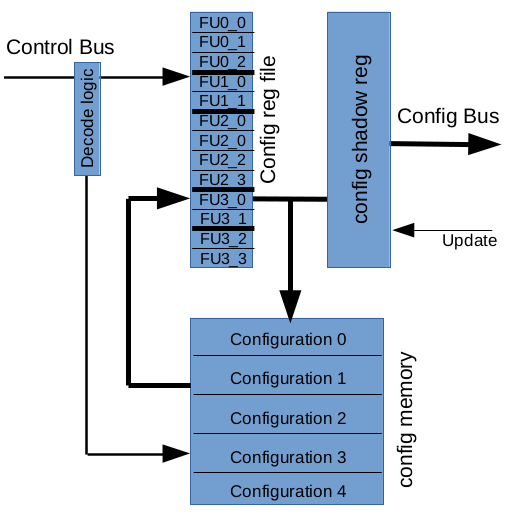
\includegraphics[width=0.8\textwidth]{drawings/conf.pdf}
\caption{Configuration Module.}
\label{fig_conf}
\end{figure}

The configuration memory is a dual-port 64-position memory, where each
position can store a full configuration and is, hence, 672 bits
wide. Configurations can be loaded/stored from/to the configuration
register file in just 1 clock cycle using one the memory ports. The
other port is 32-bit wide and used to load and store configurations in
the external memory using the DMA. This way, the configuration memory
can be extended beyond the 64 configurations. This scheme is designed
so that one can study the difference between working with pre-built
configurations stored in external memory and generating configurations
using the Versat controller.

%%%%%%%%%%%%%%%%%%%%%%%%%%%%%%%%%%%%%%%%%%%%%%%%%%%%%%%%%%%%%%%%%%%%%%%%
\section{Controller}
\label{section:controller}

The Versat Controller has a minimal architecture
(figure~\ref{fig_control}) to support reconfiguration, data movement,
algorithm control and host interaction. It contains 3 main registers:
the Program Counter (PC), the Accumulator Register (RA) and the
Address Register (RB). The PC contains the address of the next
instruction as usual. Register RA is the destination of all operations
that the controller performs, and is also often one of the operands
(accumulator architecture). Register RB is addressable by the
Controller and is used to store addresses for implementing indirect
loads and stores.

\begin{figure}[!htb]
\centering 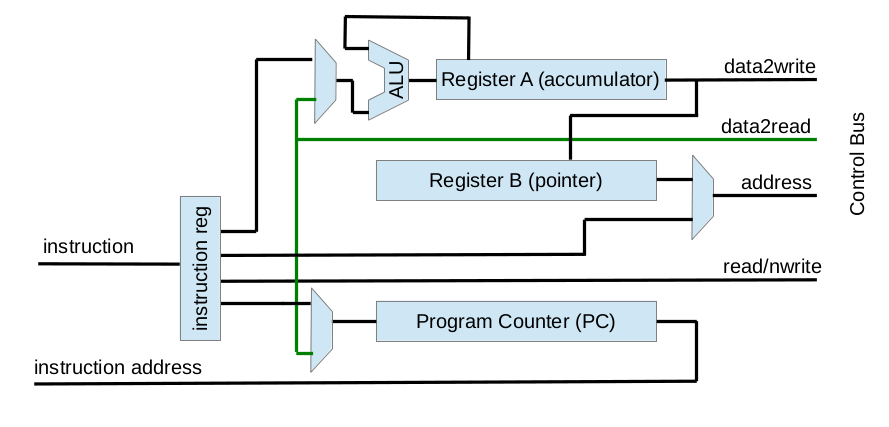
\includegraphics[width=0.95\textwidth]{drawings/control.pdf}
\caption{Controller.}
\label{fig_control}
\end{figure}

The controller has an instruction set of only 16 instructions ({\tt
  opcode} of 4 bits and {\tt Imm}ediate value of 16 bits). These allow
the controller to perform the following actions: loads/stores to/from
the accumulator, arithmetic/logic operations and branches. There are
three types of load instructions: of immediate constants, direct (from
an immediate address) and indirect from an address stored in register
RB. Store instructions can be direct or indirect.

The instruction set is outlined in Table~\ref{tab:isa}. As usual,
square brackets represent memory positions. For example, M[Imm]
represents the contents of the memory position whose address is
Imm. The PC is incremented for every instruction, except when
indicated otherwise (branch instructions).

\begin{table}[!htb]
  \renewcommand{\arraystretch}{1.2} % more space between rows
  \caption{Instruction set.}
  \label{tab:isa}
  \centering
  \begin{tabular}{cl}
    \toprule
    Instruction & Description\\
    \midrule
    nop   & No-operation\\
    rdw   & RA = M[Imm]\\
    wrw   & M[Imm] = RA\\
    rdwb  & RA = M[RB]\\
    wrwb  & M[RB] = RA\\
    beqi  & RA == 0? PC = Imm: PC += 1; RA = RA-1\\
    beq   & RA == 0? PC = M[Imm]: PC += 1; RA = RA-1\\
    bneqi & RA != 0? PC = Imm: PC += 1; RA = RA-1\\
    bneq  & RA != 0? PC = M[Imm]: PC += 1; RA = RA-1\\
    ldi   & RA = Imm\\
    ldih  & RA[31:16] = Imm\\
    shft  & RA = (Imm $<$ 0)? RA $<<$ 1: RA $>>$ 1\\
    add   & RA = RA + M[Imm]\\
    addi  & RA = RA + Imm\\
    sub   & RA = RA - M[Imm]\\
    and   & RA = RA \& M[Imm]\\
    \bottomrule
  \end{tabular}
\end{table}

In order to reduce the critical path and increase the clock frequency,
a pipeline register has been added between the instruction memory and
the instruction decoder. The controller then takes 2 clock cycles to
fetch an instruction, one from the memory itself and the other from
the instruction register shown in figure~\ref{fig_control}. For
simplicity, it executes every instruction fetched and thus branch
instructions have 2 delay slots. The delay slots can be filled with
useful instructions or with no operation (NOP) instructions.  For
instance, in a {\tt for} loop, the delay slots can be used to
increment the iteration count.

The boot loader software handles host procedure calls. The host writes
the procedure parameters to the CRF and writes the program address to
R0 which triggers a jump to the program address. During the execution
of a typical program, the DMA and the DE are used multiple times. DMA
and DE threads are spawned, hiding part of the controller execution
time, as shown later. This architecture allows programs to execute
precise time delays using a {\tt for} loop with a variable number of
instructions in its body. These instructions may be useful ones
(reconfiguration instructions, for instance) or just NOP instructions.

%%%%%%%%%%%%%%%%%%%%%%%%%%%%%%%%%%%%%%%%%%%%%%%%%%%%%%%%%%%%%%%%%%%%%%%%
\section{Divider}
\label{section:divider}

To perform divisions, Versat has a fixed-point serial divider, added
as a controller peripheral, which takes 33 cycles to complete one
division. It has shadow registers for the operands (dividend and
divisor), as well as for the results (quotient and remainder). This
means that it is possible to read the results and write next operands
while a new division is already being computed. It has one
configuration parameter that allows choosing between signed or
unsigned division. This implementation was designed for low energy and
small silicon area.

%%%%%%%%%%%%%%%%%%%%%%%%%%%%%%%%%%%%%%%%%%%%%%%%%%%%%%%%%%%%%%%%%%%%%%%%
\section{DMA}
\label{section:dma}

One of the crucial factors to guarantee acceleration is the rapidity
at which data is moved in and out of Versat. Accessing data words from
the external memory using load instructions is out of the
question. Data must be moved in large blocks using a DMA engine to
amortize the latency of the external memory device. The DMA engine is
operated by the Versat controller and transfers a data burst from
external memory into one of the Versat's memories (instruction,
configuration, or data engine memory) or vice versa.

From a Versat program point of view, the DMA is memory mapped and the
following DMA registers can be accessed: the external address
register, the internal address register, the size register, the
direction register, the status register and the start register. All
registers, except the status register, are duplicated allowing the
configuration of a new transaction while a previous one is
running. The external address register holds the transfer start
address in the external memory (32 bits), and the internal address
register holds the transfer start address in Versat (14 bits written
to a 32-bit register). The size register (8 bits) specifies the number
of words to be transferred (256 words maximum, as per the AXI4
interface). The direction register indicates if the transfer is from
Versat to external memory or vice-versa. After these registers have
been configured, the program writes anything to the start register and
the transfer begins. The contents of the status register tells the
program whether the DMA is still busy, done or if an error has
occurred.


%%%%%%%%%%%%%%%%%%%%%%%%%%%%%%%%%%%%%%%%%%%%%%%%%%%%%%%%%%%%%%%%%%%%%%%%
\section{Program memory}
\label{section:programMemory}

The Program Memory is divided in two parts: the boot ROM (256x32,
$1kB$) and the instruction memory RAM (2048x32, $8kB$). They are
addressable as a single memory: the first 256 addresses are used to
address the boot ROM, while the others are used to address the
instruction memory.

The boot ROM holds the code that allows Versat to communicate with the
host processor. Basically, it is used for the host to call Versat
kernels and to load/store values in any addressable memory position
within Versat without using the DMA. This includes loading programs
issuing store instructions to the Program Memory. However, the Program
Memory can not be read with load instructions. Its contents can only
be executed.


%%%%%%%%%%%%%%%%%%%%%%%%%%%%%%%%%%%%%%%%%%%%%%%%%%%%%%%%%%%%%%%%%%%%%%%%
\section{Control Register File}
\label{section:controlRegisterFile}

The 16x32 Control Register File (CRF) is implemented with a dual-port
register file (one port for the host and another for Versat). These
registers are shared between the host processor and Versat, which are
allowed to asynchronously read or write them.

\section{Qualitative comparison with other architectures}
\label{section:archComparisonWOtherArchitectures}

Versat has some distinctive features which can not be found in other
architectures: (1) it has a small number of FUs organized in a full
mesh structure; (2) it has a fully addressable configuration register
combined with a configuration memory to support partial configuration;
(3) it has a dedicated controller for reconfiguration, DMA management
and simple algorithm control -- no general purpose RISC~\cite{Lee00}
or VLIW~\cite{Mei05} processors are used.

CGRAs started as 1-D structures~\cite{Ebeling96} but more recently 2-D
square mesh FU arrays became more common~\cite{Lee00,Mei05,Liu15}. The
problem with square mesh topologies is that many FUs end up being used
as routing resources, reducing the number of FUs available for
computation and requiring sophisticated mapping
algorithms~\cite{Liu13}. Versat is an experiment on trading a lower FU
count with a richer interconnect structure. As explained before, the
silicon area occupied by the full mesh interconnect is less than $5\%$
and the limits placed on the frequency of operation are normally
irrelevant given the low energy budgets of target applications. In
fact, a low energy consumption often imposes a frequency of operation
which is well below Versat's maximum operating frequency.

As explained in~\cite{Liu15}, the reconfiguration time in CGRAs can
easily dominate the total execution time. To counter this effect
Versat takes partial reconfiguration to the extreme of using a fully
addressable configuration register. This keeps the reconfiguration
time to a minimum and contrasts with the more moderate hierarchical
reconfiguration scheme proposed in~\cite{Liu15}.

Since it is crucial to have reconfiguration done quickly, Versat
includes a small 16-instruction controller with low IO latency,
practically dedicated to reconfiguration management. This controller
is also used to manage data transfers and control the execution of
acceleration kernels. In other architectures~\cite{Lee00,Mei05,Liu15},
more comprehensive processors are used, which can also run complex
algorithms. However, combing complex application coding and
accelerator control is difficult. Using its controller, Versat can
completely take care of simple yet compute intensive kernels. Example
kernels are FFT, DCT, Motion Estimation, and even Big Data algorithms
such as K-Means Clustering. These kernels can simply be invoked by
host processors, and they will run in parallel to completion, without
requiring any external control.


\begin{comment}
After hardware reset the Versat, through boot ROM program, waits a
host command. Three registers of the CRF are used for this purpose:
one as a command register (R14), two as an address register (R0) and
another one as a data register (R15).

There are 3 commands (for now): read command, that allow the host to
access some data from Versat (for debug, for instance), write command,
that host uses to write some data into Versat, and run command, that
indicates to Versat to run some kernel.

In case of read, the host writes the read command into R14 (\#4), the
base address into R0 and waits that Versat write Acknowledge (Ack -
\#3) into R14. When it does, he read data from R15, clean Ack value
from R14 and waits for a new Ack. On Versat side, which is reading R0
until it has a nonzero value, after host command (written on R0), he
process the command given and get into a certain loop according the
command. In this case, after he loads the R0 value into RB, get into a
loop that reads R14 until it has a value that is not Ack. When this
happens, he checks if R14 value is equal to finish (\#2). If it is, go
back to boot ROM base address (cleans the R0 and wait it has a nonzero
value again), if not, read from the address pointed by RB, put the
data into R15, increment RB, write the Ack into R14 and go back to
read R14 loop (waits that R14 has a different value again).

In case of write, the host writes the first data value into R15, the
command into R14 and the base address into R0 (there is no write
command, it just have to be a different value that other commands uses
on protocol - i.e. \#0). When it does, he get into a loop that reads
R14 and wait for Ack. On Versat side, after processing the command
given, loads the R0 value into RB and get into a loop that reads R14
until it has a value that is not Ack. When this happens, he checks if
R14 value is equal to finish (\#2). If it is, go back to boot ROM base
address (cleans the R0 and wait it has a nonzero again), if not, write
R15 value into the address pointed by RB, increment RB, write the Ack
into R14 and go back to read R14 loop (waits that R14 has a different
value again).

For the execution of a kernel, the CRF is used by the host also to
pass parameters to Versat and by Versat to return status information
to the host (the registers used to do that are undefined, depends on
the kernel it self). After a host command, Versat do an unconditional
branch to address written on R0, starting the kernel execution.
\end{comment}
